%%%%%%%%%%%%%%%%%%%%%%%%%%%%%%%%%%%%%%%%%
% Programming/Coding Assignment
% LaTeX Template
%
% This template has been downloaded from:
% http://www.latextemplates.com
%
% Original author:
% Ted Pavlic (http://www.tedpavlic.com)
%
% Note:
% The \lipsum[#] commands throughout this template generate dummy text
% to fill the template out. These commands should all be removed when 
% writing assignment content.
%
% This template uses a Perl script as an example snippet of code, most other
% languages are also usable. Configure them in the "CODE INCLUSION 
% CONFIGURATION" section.
%
%%%%%%%%%%%%%%%%%%%%%%%%%%%%%%%%%%%%%%%%%

%----------------------------------------------------------------------------------------
%	PACKAGES AND OTHER DOCUMENT CONFIGURATIONS
%----------------------------------------------------------------------------------------

\documentclass{article}

\usepackage{fancyhdr} % Required for custom headers
\usepackage{lastpage} % Required to determine the last page for the footer
\usepackage{extramarks} % Required for headers and footers
\usepackage[usenames,dvipsnames]{color} % Required for custom colors
\usepackage{graphicx} % Required to insert images
\usepackage{listings} % Required for insertion of code
\usepackage{courier} % Required for the courier font
\usepackage{lipsum} % Used for inserting dummy 'Lorem ipsum' text into the template

% Margins
\topmargin=-0.45in
\evensidemargin=0in
\oddsidemargin=0in
\textwidth=6.5in
\textheight=9.0in
\headsep=0.25in

\linespread{1.1} % Line spacing

% Set up the header and footer
\pagestyle{fancy}
\lhead{\hmwkAuthorName} % Top left header
\chead{\hmwkClass\ (\hmwkClassInstructor\ \hmwkClassTime): \hmwkTitle} % Top center head
\rhead{\firstxmark} % Top right header
\lfoot{\lastxmark} % Bottom left footer
\cfoot{} % Bottom center footer
\rfoot{Page\ \thepage\ of\ \protect\pageref{LastPage}} % Bottom right footer
\renewcommand\headrulewidth{0.4pt} % Size of the header rule
\renewcommand\footrulewidth{0.4pt} % Size of the footer rule

\setlength\parindent{0pt} % Removes all indentation from paragraphs

%----------------------------------------------------------------------------------------
%	CODE INCLUSION CONFIGURATION
%----------------------------------------------------------------------------------------

\definecolor{MyDarkGreen}{rgb}{0.0,0.4,0.0} % This is the color used for comments
\lstloadlanguages{Perl} % Load Perl syntax for listings, for a list of other languages supported see: ftp://ftp.tex.ac.uk/tex-archive/macros/latex/contrib/listings/listings.pdf
\lstset{language=Perl, % Use Perl in this example
        frame=single, % Single frame around code
        basicstyle=\small\ttfamily, % Use small true type font
        keywordstyle=[1]\color{Blue}\bf, % Perl functions bold and blue
        keywordstyle=[2]\color{Purple}, % Perl function arguments purple
        keywordstyle=[3]\color{Blue}\underbar, % Custom functions underlined and blue
        identifierstyle=, % Nothing special about identifiers                                         
        commentstyle=\usefont{T1}{pcr}{m}{sl}\color{MyDarkGreen}\small, % Comments small dark green courier font
        stringstyle=\color{Purple}, % Strings are purple
        showstringspaces=false, % Don't put marks in string spaces
        tabsize=5, % 5 spaces per tab
        %
        % Put standard Perl functions not included in the default language here
        morekeywords={rand},
        %
        % Put Perl function parameters here
        morekeywords=[2]{on, off, interp},
        %
        % Put user defined functions here
        morekeywords=[3]{test},
       	%
        morecomment=[l][\color{Blue}]{...}, % Line continuation (...) like blue comment
        numbers=left, % Line numbers on left
        firstnumber=1, % Line numbers start with line 1
        numberstyle=\tiny\color{Blue}, % Line numbers are blue and small
        stepnumber=5 % Line numbers go in steps of 5
}

% Creates a new command to include a perl script, the first parameter is the filename of the script (without .pl), the second parameter is the caption
\newcommand{\perlscript}[2]{
\begin{itemize}
\item[]\lstinputlisting[caption=#2,label=#1]{#1.pl}
\end{itemize}
}

%----------------------------------------------------------------------------------------
%	DOCUMENT STRUCTURE COMMANDS
%	Skip this unless you know what you're doing
%----------------------------------------------------------------------------------------

% Header and footer for when a page split occurs within a problem environment
\newcommand{\enterProblemHeader}[1]{
\nobreak\extramarks{#1}{#1 continued on next page\ldots}\nobreak
\nobreak\extramarks{#1 (continued)}{#1 continued on next page\ldots}\nobreak
}

% Header and footer for when a page split occurs between problem environments
\newcommand{\exitProblemHeader}[1]{
\nobreak\extramarks{#1 (continued)}{#1 continued on next page\ldots}\nobreak
\nobreak\extramarks{#1}{}\nobreak
}

\setcounter{secnumdepth}{0} % Removes default section numbers
\newcounter{homeworkProblemCounter} % Creates a counter to keep track of the number of problems

\newcommand{\homeworkProblemName}{}
\newenvironment{homeworkProblem}[1][Problem \arabic{homeworkProblemCounter}]{ % Makes a new environment called homeworkProblem which takes 1 argument (custom name) but the default is "Problem #"
\stepcounter{homeworkProblemCounter} % Increase counter for number of problems
\renewcommand{\homeworkProblemName}{#1} % Assign \homeworkProblemName the name of the problem
\section{\homeworkProblemName} % Make a section in the document with the custom problem count
\enterProblemHeader{\homeworkProblemName} % Header and footer within the environment
}{
\exitProblemHeader{\homeworkProblemName} % Header and footer after the environment
}

\newcommand{\problemAnswer}[1]{ % Defines the problem answer command with the content as the only argument
\noindent\framebox[\columnwidth][c]{\begin{minipage}{0.98\columnwidth}#1\end{minipage}} % Makes the box around the problem answer and puts the content inside
}

\newcommand{\homeworkSectionName}{}
\newenvironment{homeworkSection}[1]{ % New environment for sections within homework problems, takes 1 argument - the name of the section
\renewcommand{\homeworkSectionName}{#1} % Assign \homeworkSectionName to the name of the section from the environment argument
\subsection{\homeworkSectionName} % Make a subsection with the custom name of the subsection
\enterProblemHeader{\homeworkProblemName\ [\homeworkSectionName]} % Header and footer within the environment
}{
\enterProblemHeader{\homeworkProblemName} % Header and footer after the environment
}

%----------------------------------------------------------------------------------------
%	NAME AND CLASS SECTION
%----------------------------------------------------------------------------------------

\newcommand{\hmwkTitle}{FE-Assignment\ \#07} % Assignment title
\newcommand{\hmwkDueDate}{Monday,\ March\ 14,\ 2016} % Due date
\newcommand{\hmwkClass}{MA\ 374} % Course/class
\newcommand{\hmwkClassTime}{} % Class/lecture time
\newcommand{\hmwkClassInstructor}{} % Teacher/lecturer
\newcommand{\hmwkAuthorName}{Silvi Pandey (130123045)} % Your name

%----------------------------------------------------------------------------------------
%	TITLE PAGE
%----------------------------------------------------------------------------------------

\title{
\vspace{2in}
\textmd{\textbf{\hmwkClass:\ \hmwkTitle}}\\
\normalsize\vspace{0.1in}\small{Due\ on\ \hmwkDueDate}\\
\vspace{0.1in}\large{\textit{\hmwkClassInstructor\ \hmwkClassTime}}
\vspace{3in}
}

\author{\textbf{\hmwkAuthorName}}
\date{} % Insert date here if you want it to appear below your name

%----------------------------------------------------------------------------------------

\begin{document}

\maketitle

%----------------------------------------------------------------------------------------
%	TABLE OF CONTENTS
%----------------------------------------------------------------------------------------

%\setcounter{tocdepth}{1} % Uncomment this line if you don't want subsections listed in the ToC

\newpage

\begin{center}
\textbf{PROBLEM 1}
\end{center}
Assume $T = 1, K = 1, r = 0.05, \sigma = 0.6$. Plot, in a single graph, $C(t, s)$ as a function of $s$ alone for
$t = 0, 0.2, 0.4, 0.6, 0.8, 1$. Do a similar plot for $P(t, s)$ as a function of $s$. Now, show the same information in a
3-dimensional form, i.e., as a function both t and s.

\begin{center}
\textbf{SOLUTION}
\end{center}

Under the BSM framework the price of European put and call options as a function of the time and the stock price is given by :
\begin{center}
\includegraphics[width=80mm]{Formula}
\end{center}
In the above expression the respective variables represent :\\
(1) N(x) is the cumulative distribution function of the standard normal distribution\\
(2) T - t is the time to maturity\\
(3) S is the spot price of the underlying asset\\
(4) K is the strike price\\
(5) r is the risk free rate (annual rate, expressed in terms of continuous compounding)\\
(6) $\sigma$ is the volatility of returns of the underlying asset\\

\textbf{(1) European Call}
\begin{center}
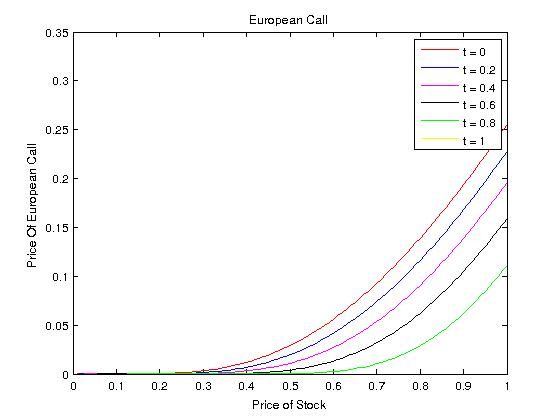
\includegraphics[width=70mm]{Call1}
\end{center}

\textbf{(2) European Put}
\begin{center}
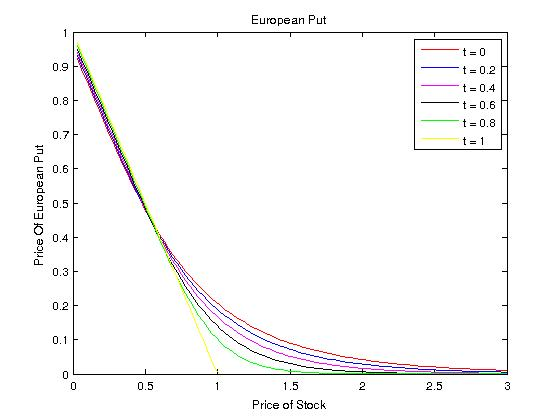
\includegraphics[width=70mm]{Put1}
\end{center}

When the values for the spot price of the stock is higher, the curve almost becomes a straight line as observed in the following plots.

\textbf{(1) European Call}
\begin{center}
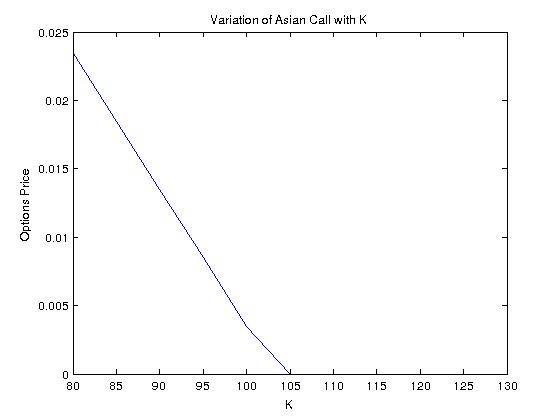
\includegraphics[width=70mm]{Call}
\end{center}

\textbf{(2) European Put}
\begin{center}
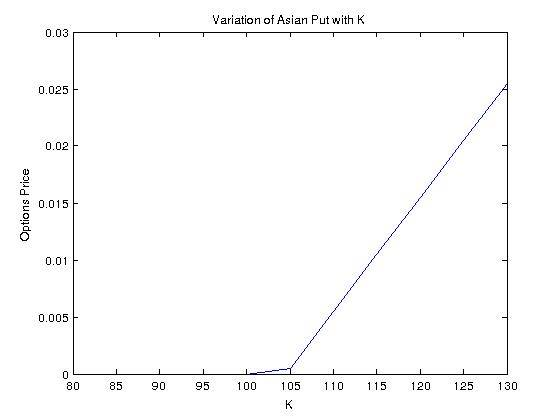
\includegraphics[width=70mm]{Put}
\end{center} 

\begin{center}
\textbf{PROBLEM 2}
\end{center}
Plot $C(t, s)$ and $P(t, s)$ as a smooth surface above the $(t, s)$-plane.

\begin{center}
\textbf{SOLUTION}
\end{center}

The following plots were obtained :\\
\textbf{(1) 3D - European Call}
\begin{center}
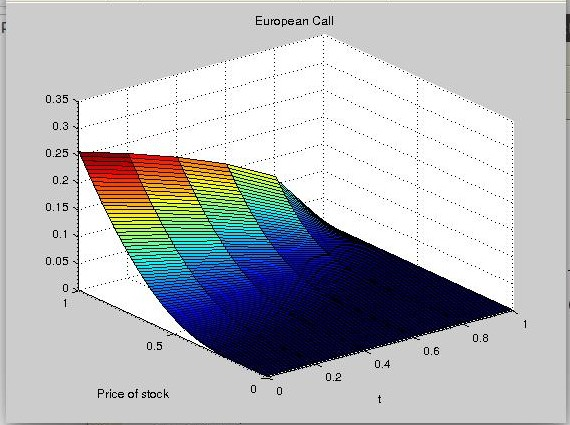
\includegraphics[width=70mm]{Call3D}
\end{center}

\textbf{(2) 3D - European Put}
\begin{center}
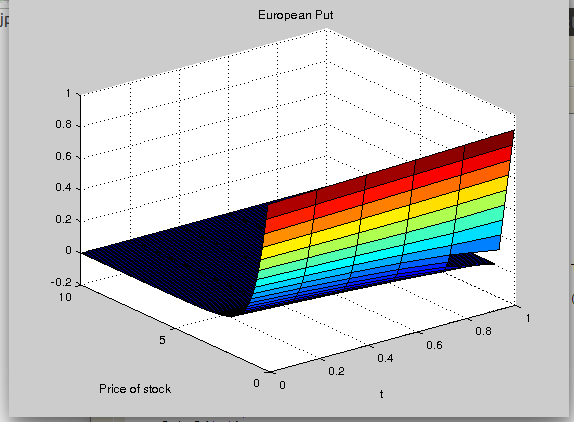
\includegraphics[width=70mm]{Put3D}
\end{center}

\begin{center}
\textbf{PROBLEM 3}
\end{center}
Study the sensitivity of both the functions C and P as a function of model parameters. If required, you may
assume different parameter values as opposed to the one given above. Present your results in the form of tables
and graphs (both in two and three dimensional).

\begin{center}
\textbf{SOLUTION}
\end{center}
The model parameters are $\sigma$ , $K$ and $r$. In order to do sensitivity analysis on all of them , the spot price was fixed to 0.05 and the individual parameters were varied with respect to the values of time given in the problem.The following plots were obtained by varying each parameter with time for both call and put options.\\

\textbf{(1) Varying $\sigma$}\\
European Call Option :
\begin{center}
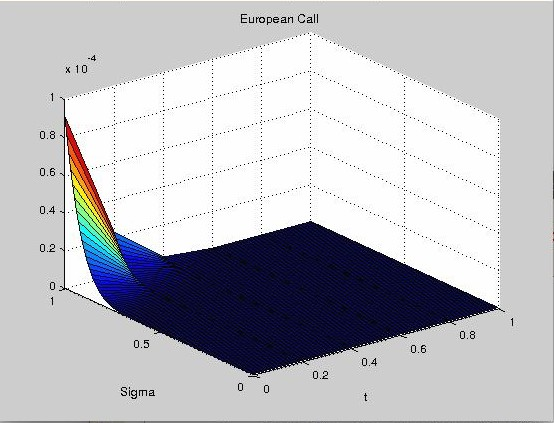
\includegraphics[width=65mm]{CallVary_sigma}
\quad \quad
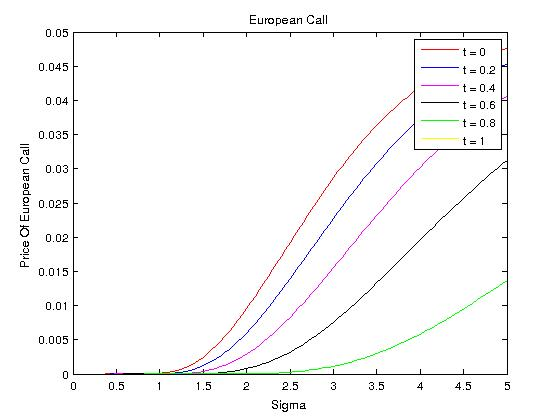
\includegraphics[width=65mm]{CallVary_sigma2D}
\end{center}

European Put Option :
\begin{center}
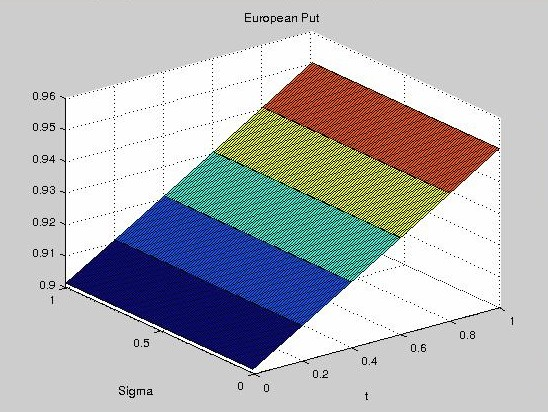
\includegraphics[width=65mm]{PutVary_sigma}
\quad \quad
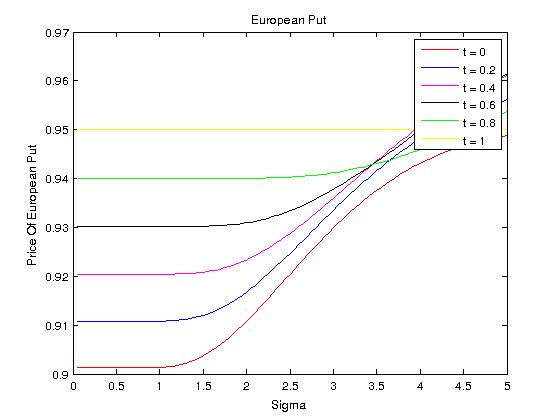
\includegraphics[width=65mm]{PutVary_sigma2D}\\
\end{center}

\textbf{(2) Varying $r$}\\\\
European Call Option :
\begin{center}
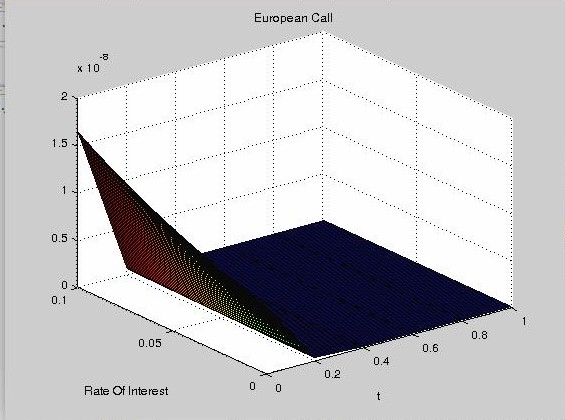
\includegraphics[width=65mm]{CallVary_r}
\quad \quad
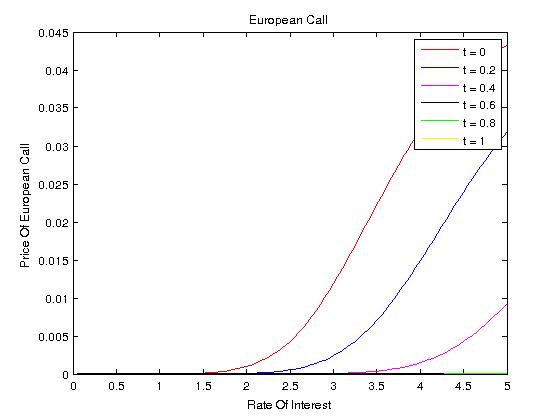
\includegraphics[width=65mm]{CallVary_r2D}\\
\end{center}

European Put Option :
\begin{center}
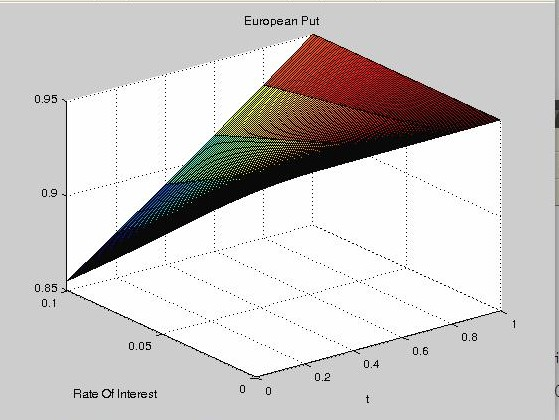
\includegraphics[width=65mm]{PutVary_r}
\quad \quad
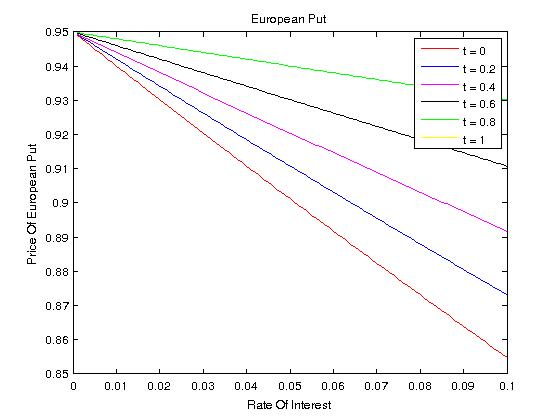
\includegraphics[width=65mm]{PutVary_r2D}\\
\end{center}

\textbf{(3) Varying $K$}\\\\
European Call Option :
\begin{center}
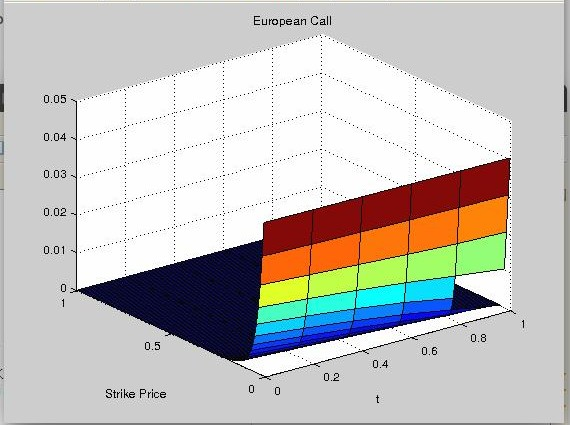
\includegraphics[width=65mm]{CallVary_K}
\quad \quad
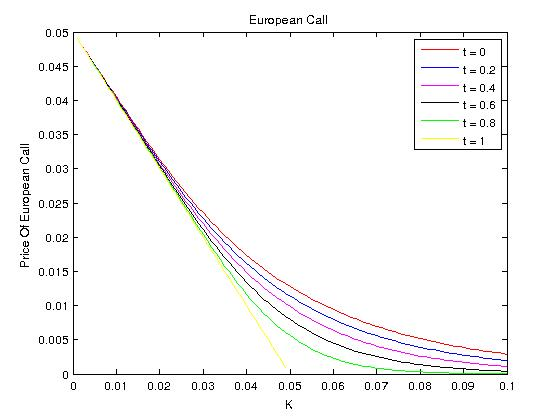
\includegraphics[width=65mm]{CallVary_K2D}\\
\end{center}
\newpage
European Put Option :
\begin{center}
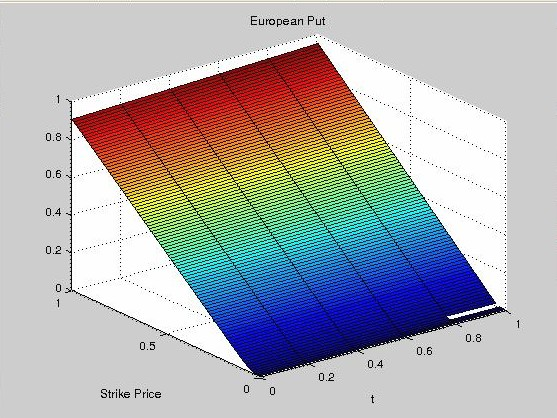
\includegraphics[width=65mm]{PutVary_K}
\quad \quad
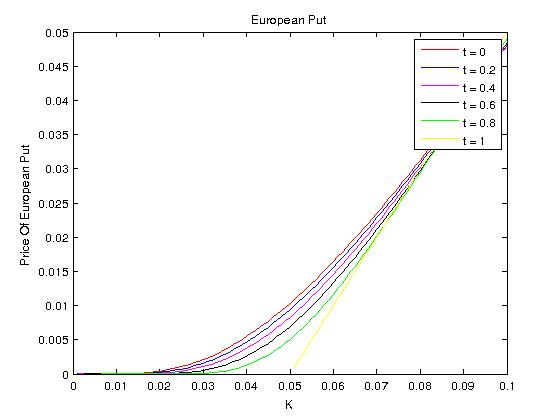
\includegraphics[width=65mm]{PutVary_K2D}
\end{center}

\textbf{Observations}\\
(1) The price Of European Call option increases with the increase in the spot price of the stock. With increase in the stock price, the holder of the call option ( long the call ) will have more profit, as the holder can buy the stock at a comparatively lesser price than the the actual market price of the stock by exercising the option. The price of the European Put option decreases with the increase in the spot price because of analogous reason.\\
(2) The prices of both European Call and put options increase with increase in the volatility of the stock \\
(3) The price of European Call option increases with the increase in the risk free rate because with increase in r, the spot price increases as the stock price process  is a GBM and increase with $\mu$ (r).Analogous reason for decrease in the price of European Put with increase in r.\\
(4) The price of European Call option decreases with increase in K because with increase in K, the holder of call (long the call) will have less profit and analogously for European Put option.


\end{document}